\section{An overview of $\Delta$QSD}
    $\Delta$QSD is a metrics-based, quality-centric paradigm that uses formalised outcome diagrams to explore the performance consequences of design decisions. \cite{myo}
    
    Key concepts of $\Delta$QSD are \textbf{quality attenuation ($\Delta$Q)} and \textbf{outcome diagram} \cite{dq-tut}.

    Outcome diagrams capture dependency and causality properties of the system. The $\Delta$QSD paradigm derives bounds on performance expressed as probability distribution, encompassing all possible executions of the system. \cite{myo}
 
    The following sections are a summary of multiple articles and presentation formalising the paradigm.
     
 \subsection{Outcome}
           An outcome $o$ is a specific system behaviour that can be observed to start at some point in time and \textit{\textbf{may}} be observed to complete at some later time. \cite{dq-br}
        Formally, what the system obtains by performing one of its tasks. One task corresponds to one outcome and viceversa. When an outcome is performed, it means that the task of an outcome is performed.
     
        The particularity of outcomes is that they can represent multiple levels of granularity, suppose an outcome may be beyond the current system's control (e.g. a database/cloud request), is non-atomic (can be broken down in multiple sub-outcomes). These outcomes can be represented as black-boxes, as the system gets refined, these outcomes can then be modeled by multiple outcomes. \\ 
        Even though these outcomes are defined as "black boxes", they still have timeliness constraints like any other outcome. \cite{myo}

     \paragraph{Observables}
    Each outcome has two starting sets of events: the starting sets and the ending sets. Such sets are called the \textit{observables}. Once an event from the starting set occurs, there is no guarantee that a corresponding event in the terminating set will occur within the duration limit (required time to complete). An observable is \textit{done}  when it occurs during the time limit. \cite{art}

    \paragraph{Outcome instance}
    An outcome instance is the result of an execution of an outcome given a starting event $e_{in}$ and an end event $e_{out}$. \cite{art}

    \paragraph{Graphical Representation}
    Outcomes are represented as circles, with the starting and terminating set of events being represented by boxes.
    \begin{figure}[H]
        \begin{center}
            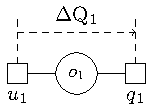
\includegraphics[scale=1.2]{tikz/outdq.pdf}
        \end{center}
        \caption{The outcome (circle) and the starting set (left) and terminating set (right) of events. \cite{myo}}
    \end{figure}

\subsection{Quality attenuation ($\Delta$Q)}
        Assume a component $C$ which receives a message $m_{in}$ and outputs a message $m_{out}$ after a delay $d$. Over multiple executions, we will have observed multiple delays which can be represented as a cumulative definition where $p$ percent of delays have delay $\le d$. \cite{art} 

        \textbf{$\Delta$Q} is a cumulative distribution function that defines both \textit{latency} and \textit{failure probability} between a start and end event. \cite{dq-tut}

        In an ideal system, an outcome would deliver a desired behaviour without error, failure, delay, but this is not the case. The quality of an outcome response "attenuated to the relative ideal" (the cumulative distribution function) is called "quality attenuation" ($\Delta$Q) and can depend on many factors (geographical, physical \dots). Its distribution may be modelled by a random variable.

    As $\Delta$Q captures deviation from ideal behavior and incorporates delay, which is a continuous random variable, and failures/timeouts, which are discrete variables, it can be described mathematically as an \textit{Improper Random Variable}, where the probability of a finite or bounded delay $<$ 1. Combining latency and failure together makes it easy to examine the tradeoffs between them.

    \textbf{$\Delta$Q(x)} is the probability that an outcome $O$ occurs in time $t \le x$. The \textbf{\textit{intangible mass}} $1 - \lim_{x\to\infty}\Delta Q(x)$ of a $\Delta$Q will encode the probability of failure/timeout/exception occuring. \cite{myo}
    
    \begin{figure}[H]
        \begin{center}
            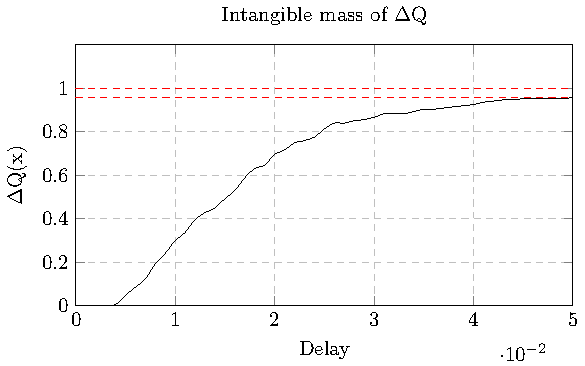
\includegraphics{tikz/intangible.pdf}
        \end{center}
        \caption{Intangible mass (red) of a $\Delta$Q with failure rate of about 5\% }
    \end{figure}
   
  \subsection{Failure semantics}
       In the CDF representation of a $\Delta$Q, there is an \textit{f} percent probability that the delay is infinite, this is what failure models. 
        Concretely, it means that an input message $m_{in}$ \textbf{has no output message} $m_{out}$. \cite{art}

        Combining delay and failure in a single quantity is what makes $\Delta$QSD a great choice to explore feasibility in system design. \cite{dq-tut}
   
    \subsection{Partial ordering}
        A CDF of a $\Delta$Q is \textit{less than} the other if its CDF is everywhere to the left and above the other. Mathematically, it is a partial order. 
        
        If two $\Delta$Qs intersect, they are not ordered. \cite{dq-tut}

    \subsection{Timeliness}
        Timeliness is defined as a relation between an observed $\Delta Q_{obs}$ and a required $\Delta Q_{req}$. Timeliness is delivering results within required time bounds (sufficiently often). 

        A system \textit{satisfies timeliness} if $\Delta$Q$_{obs}$ $\le$ $\Delta$Q$_{req}$. \cite{art}
     
    \subsection{QTA, required $\Delta$Q}
         The \textit{Quantitative Timeliness Agreement} (QTA) maps objective measurements to the subjective perception of application performance. It specifies what the base system does and its limits. \cite{dq-br} \cite{myo}
    
    \paragraph{Slack} There is performance \textit{slack} when a $\Delta$Q is strictly less than the requirement,

        \paragraph{Hazard} There is performance \textit{hazard} when a $\Delta$Q is strictly greater than the requirement.
    
    \paragraph{QTA example}: Imagine a system where 25\% of the executions should take $<$ 15 ms, 50\% $<$ 25 ms and 75\% $<$ 35 ms, all queries have a maximum delay of 50ms and 5\% of executions can timeout, the QTA can be represented as a step function.
    
        \begin{figure}[H]
            \begin{center}
                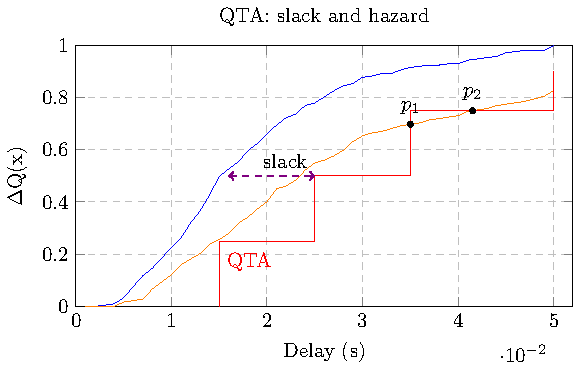
\includegraphics[scale=1]{tikz/cdf_qta_slack.pdf}
            \end{center}
            \caption{The system in blue is showing slack and satisfies the requirement. The system in orange is showing signs that it cannot handle the stress, it is not respecting the system requirements imposed by the QTA.}%
        \end{figure}

    \subsection{Outcome diagram}
        An outcome diagram is central to capture the causal relationships between the outcomes. It shows the causal connections between all the outcomes we are interested in, and it allows computing the $\Delta$Q for the whole system \cite{dq-tut}. It maps a system's behaviour as seen from outside to concrete outcomes \cite{art}.
        There are four different operators that represent the relationships between outcomes. \cite{dq-tut}

    \subsubsection{Sequential composition}
        If we assume two outcomes $O_A$, $O_B$ where the end event of $O_A$ is the start event of $O_B$, the two outcomes can be sequentially composed. The total delay $\Delta$Q$_{AB}$ is given by the convolution of the PDFs of $O_A$ and $O_B$ ($O_A \circledast O_B$).
        
        \begin{figure}[H]
            \begin{center}
                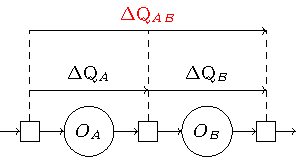
\includegraphics[scale=1]{tikz/seq_comp.pdf}
            \end{center}
            \caption{Sequential composition of $O_A$ and $O_B$.}
        \end{figure}
        Where convolution ($\circledast$) between two PDF is:
        \begin{equation}
            PDF_{AB}(t) =\int\limits_0^t PDF_A(\delta) \cdot PDF_B(t-\delta)d\delta 
            \label{eq:conv_1}
        \end{equation}

        Thus, $\Delta$Q$_{AB}$:
        \begin{equation}
            \Delta Q_{AB} = PDF_{A} \circledast PDF_{B}
            \label{eq:convolution_pdf}
        \end{equation}

        Convolution is the only operation which is based on the PDFs, the following operations are based on the CDF of the $\Delta$Qs (hence the use of the $\Delta$Q notation).
        
    \subsubsection{First to finish (FTF)}
            If we assume two independent outcomes $O_A$, $O_B$ with the same start event, first-to-finish occurs when at least one end event occurs, it can be calculated as:
        \begin{equation}
            \begin{split}
                \Delta Q_{FTF(A, B)} &= Pr[d_A > t \wedge d_B > t] \\
                & = Pr[d_A > t] \cdot Pr[d_B > t] = (1 - \Delta Q_A) \cdot (1 - \Delta Q_B) \\
                \Delta Q_{FTF(A, B)} &= \Delta Q_A + \Delta Q_B - \Delta Q_A \cdot \Delta Q_B  
            \end{split}    
            \label{eq:ftf} 
        \end{equation}

       \begin{figure}[H]
            \centering
            \begin{subfigure}{.5\textwidth}
                \centering
                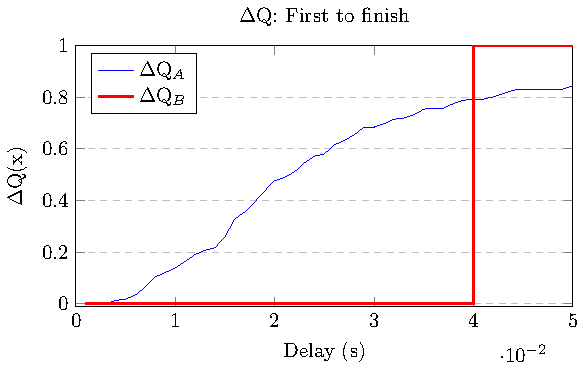
\includegraphics[scale = 0.7]{tikz/ftf_1.pdf}
                \label{fig:ftf1}
            \end{subfigure}%
            \begin{subfigure}{.5\textwidth}
                \centering
                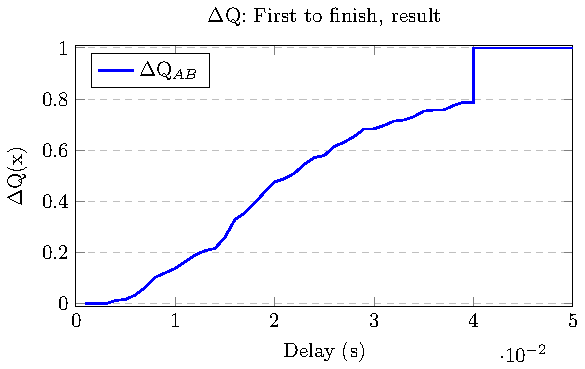
\includegraphics[scale = 0.7]{tikz/ftf_2.pdf}
                \label{fig:ftf2}
            \end{subfigure}
            \caption{Left: $\Delta$Q$_{(A, B)}$. Right: FTF$_{(A, B)}$ = $\Delta$Q$_{AB}$}%
            \label{fig:ftf}
            \end{figure}


    \subsubsection{All to finish (ATF)}
        If we assume two independent outcomes $O_A$, $O_B$ with the same start event, all-to-finish occurs when both end events occur, it can be calculated as:
        \begin{equation}
            \begin{split}
                \Delta Q_{ATF(A, B)} &= Pr[d_A \le t \wedge d_B \le t] \\
                & = Pr[d_A \le t] \cdot Pr[d_B \le t] = \Delta Q_A \cdot \Delta Q_B \\
                \Delta Q_{ATF(A, B)} &= \Delta Q_A \cdot \Delta Q_B 
            \end{split}
            \label{eq:atf}
        \end{equation}
        
        \begin{figure}[H]
            \centering
            \begin{subfigure}{.5\textwidth}
                \centering
                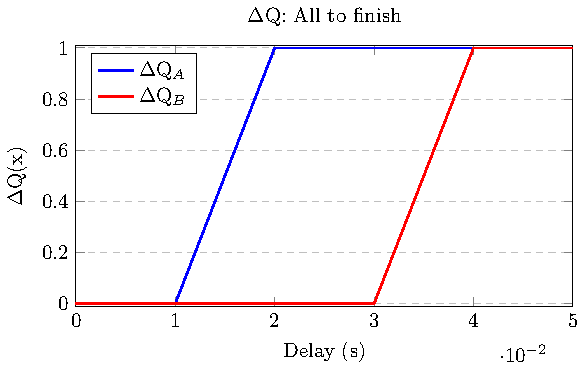
\includegraphics[scale = 0.7]{tikz/atf_1.pdf}
                \label{fig:atf_1}
            \end{subfigure}%
            \begin{subfigure}{.5\textwidth}
                \centering
                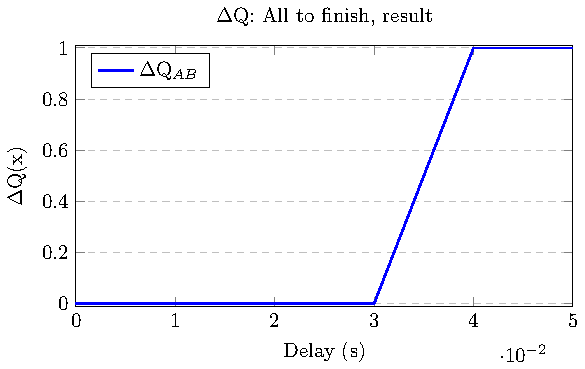
\includegraphics[scale = 0.7]{tikz/atf_2.pdf}
                \label{fig:atf2}
            \end{subfigure}
            \caption{Left: $\Delta$Q$_{(A, B)}$. Right: ATF$_{(A, B)}$ = $\Delta$Q$_{AB}$}%
            \label{fig:atf}
            \end{figure}

    \subsubsection{Probabilistic choice (PC)}
        If we assume two possible outcomes $O_A$ and $O_B$ and exactly one outcome is chosen during each occurence of a start event and:
        \begin{itemize}
            \item $O_A$ happens with probability $\dfrac{p}{p+q}$
            \item $O_B$ happens with probability $\dfrac{q}{p + q}$
        \end{itemize}
        \begin{equation}
           \Delta Q_{PC}(A, B) = \dfrac{p}{p + q}\Delta Q_A + \dfrac{q}{p + q}\Delta Q_B 
            \label{eq:pc}
        \end{equation} 

    \begin{figure}[H]
        \begin{center}
            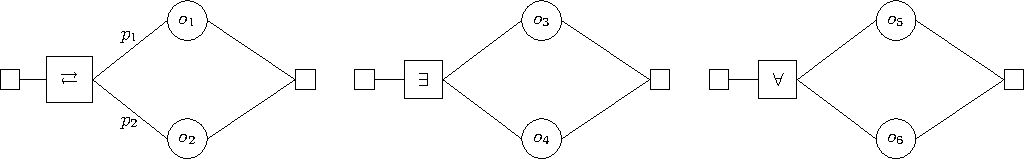
\includegraphics[width = \textwidth]{tikz/op.pdf}
        \end{center}
        \caption{The possible operators in an outcome diagram: Probabilistic choice, first-to-finish, all-to-finish}
        \label{fig:op}
    \end{figure}
    First-to-finish, All-to-finish and probabilistic-choice are calculated on the CDF of the $\Delta$Q of their components.
    
    These operators can be assembled together to create an outcome diagram, later on, we will see how one can go from the graphical representation to outcome diagrams which can be used in the $\Delta$Q oscilloscope.
    
    \subsection{Outcome diagrams refinement}
        An important feature of outcome diagrams is the ability to be able to design a system even with \textit{"black-boxes"}, before the complete details of it are known. \\
        An outcome diagram can be "unboxed" by refining the outcomes that compose it. We can adapt a situation described in Mind your Outcomes to understand how refinement can allow the user to have a very precise representation of a system. \cite{myo}
        
        We first start with a black-box, unnamed outcome with start event $A$ and end event $Z$, somewhere in the system. The first refinement step would be giving the outcome a name.

      \begin{figure}[H]
            \begin{center}
                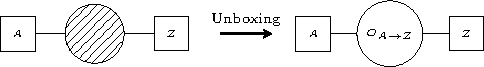
\includegraphics[scale = 1]{tikz/black_box.pdf}
            \end{center}
            \caption{Refinement from black box to named outcome.}
            \label{fig:bb}
        \end{figure}

    The system can be further refined by adding outcomes that represent tasks. For example, the engineer might believe that it will take two tasks to get from A to Z. We can then add another outcome, sequentially composed, to represent this situation.

       \begin{figure}[H]
            \begin{center}
                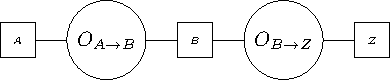
\includegraphics[scale = 1]{tikz/out_2.pdf}
            \end{center}
            \caption{Further refinement from one task to two tasks.}
            \label{fig:2_hops}
        \end{figure}

        We can also model the chance of executing two tasks as a probabilistic choice, where there is p2 probability that the execution from A to Z will execute two tasks. The outcome diagram can be refined as a probabilistic choice.

   \begin{figure}[H]
            \begin{center}
                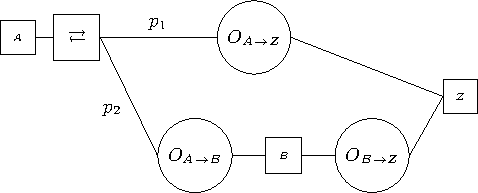
\includegraphics[scale = 1]{tikz/ref_op.pdf}
            \end{center}
            \caption{Refinement as probabilistic choice of executing either one or two tasks.}
            \label{fig:prob_ref}
        \end{figure}
    In essence, the refinement could model a very fine-grained representation of the system by further refining the system. The model could be further refined to represent the probability of executing $n$ tasks. This represents the power of outcome diagrams to represent system diagrams with high precision.
    \subsection{Independence hypothesis}    
        Assume two sequentially composed outcomes $o_1$, $o_2$ running on the same processor. The delay of execution can be observed from the start event of $o_1$ to the end event of $o_2$. 
        \begin{figure}[H]
            \begin{center}
                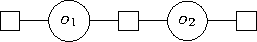
\includegraphics[scale=1]{tikz/indep.pdf}
            \end{center}
        \end{figure}
        
        At low load, the two components behavior will be independent, the system will behave linearly, the observed total delay of execution will be equal to the result of convolution of $o_1$, $o_2$ ($o_1 \circledast o_2$).
        
        When load increases, the two components will start to show dependent behaviour due to the processor utilisation increasing. The $\Delta$Q of the observed delay will then deviate from the $\Delta$Q which is the result of the convolution of $o_1, o_2$
        
        \begin{figure}[H]
            \begin{center}
                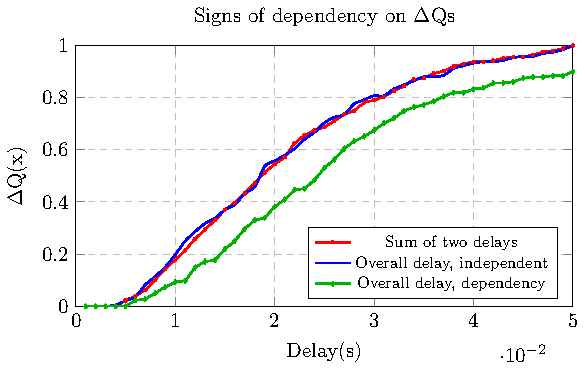
\includegraphics[scale=1]{tikz/cdf_indep.pdf}
            \end{center}
            \caption{When the components are independent, what is observed (blue) and calculated (red) can be superposed, whilst when $o_1$ and $o_2$ show initial signs of dependency, what is observed (green) can be seen deviating from the $\Delta$Q$_{o1, o2}$.}
            \label{fig:cdf_indep}
        \end{figure}

        When the system is far from being overloaded, the effect is noticeable thanks to $\Delta$QSD even if the system is far from being overloaded. As the cliff edge of overload is approached, the nonlinearity will increase \cite{post}. These theoretical results can be observed in practice in the oscilloscope.
